\documentclass{standalone}
\usepackage{tikz}
\usepackage{circuitikz}

\begin{document}
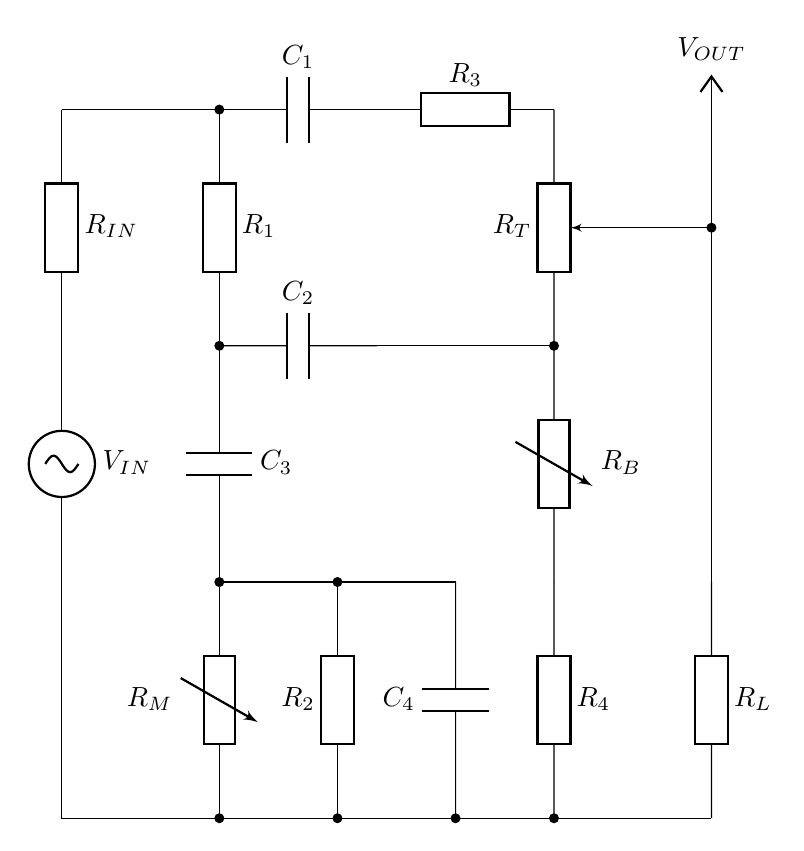
\begin{tikzpicture}
	\draw (2, 7) to[sinusoidal voltage source, l=$V_{IN}$] (2, 4);

	\draw (2, 10) to[european resistor, l=$R_{IN}$] (2, 7);
	\draw (4, 10) to[european resistor, l=$R_1$] (4, 7);
	\draw (5.5, 4) to[european resistor, l_=$R_2$] (5.5, 1);
	\draw (6, 10) to[european resistor, l=$R_3$] (8.25, 10);
	\draw (8.25, 4) to[european resistor, l=$R_4$] (8.25, 1);
	\draw (10.25, 4) to[european resistor, l=$R_L$] (10.25, 1);

	\draw (8.25, 7) to[variable european resistor, l=$R_B$] (8.25, 4);
	\draw (4, 4) to[variable european resistor, l_=$R_M$] (4, 1);
	\draw (8.25, 10) to[european potentiometer, l_=$R_T$] (8.25, 7);

	\draw (4, 10) to[capacitor, l=$C_1$] (6, 10);
	\draw (4, 7) to[capacitor, l=$C_2$] (6, 7);
	\draw (4, 7) to[capacitor, l=$C_3$] (4, 4);
	\draw (7, 4) to[capacitor, l_=$C_4$] (7, 1);

	\draw (2, 4) -- (2, 1) -| (10.25, 1);
	\draw (2, 10) -- (4, 10);
	\draw (7, 4) -- (4, 4);
	\draw (6, 7) -- (8.25, 7);
	\draw (8.75, 8.5) -- (10.25, 8.5);
	\draw (10.25, 10) -- (10.25, 8.5);
	\draw (10.25, 4) -- (10.25, 8.5);

	\node[vcc] at (10.25, 10) {$V_{OUT}$};
	\node[circ] at (10.25, 8.5) {};
	\node[circ] at (4, 1) {};
	\node[circ] at (4, 10) {};
	\node[circ] at (4, 4) {};
	\node[circ] at (4, 7) {};
	\node[circ] at (5.5, 1) {};
	\node[circ] at (5.5, 4) {};
	\node[circ] at (7, 1) {};
	\node[circ] at (8.25, 1) {};
	\node[circ] at (8.25, 7) {};

\end{tikzpicture}
\end{document}